 %=================================================================
\documentclass[metals,article,submit,moreauthors,pdftex,10pt,a4paper]{Definitions/mdpi} 
\usepackage{siunitx}
\usepackage{multirow}
\preto{\abstractkeywords}{\nolinenumbers}
\firstpage{1} 
\makeatletter 
\setcounter{page}{\@firstpage} 
\makeatother
\pubvolume{xx}
\issuenum{1}
\articlenumber{5}
\pubyear{2018}
\copyrightyear{2018} 
%\externaleditor{Academic Editor: name}
\history{Received: date; Accepted: date; Published: date}
 
% Full title of the paper (Capitalized)
% \Title{Effect of Nanovoid on Fracture Process of Two-Phase $\gamma$($\rm TiAl$)+$\alpha_2$($\rm Ti_3Al$) Alloy}
\Title{Micromechanism of  Cold Deformation of Two Phase Polycrystalline Ti-Al Alloy with and without Void Defect}
% Author Orchid ID: enter ID or remove command
\newcommand{\orcidauthorA}{0000-0001-8385-4439} % Add \orcidA{} behind the author's name
\newcommand{\orcidauthorB}{0000-0002-9582-6301} % Add \orcidB{} behind the author's name

% Authors, for the paper (add full first names)
\Author{Author \orcidA{}}
%\Author{Ruicheng Feng $^{1,2}$\orcidA{}, Maomao Wang $^{1}$\orcidB{}}

% Authors, for metadata in PDF
%\AuthorNames{Maomao Wang $^{1,\dagger,\ddagger}$\orcidB{}, Firstname Lastname and Firstname Lastname}

% Affiliations / Addresses (Add [1] after \address if there is only one affiliation.)
\address{%
% $^{1}$ \quad School of Mechanical and Electronical Engineering, Lanzhou University of Technology, Lanzhou 730050, China; frcly@163.com (R.F.); 15620864891@163.com (M.W.)\\
$^{1}$ \quad School of Mechanical and Electronical Engineering, Lanzhou University of Technology, Lanzhou 730050, China;\\
% $^{2}$ \quad Key Laboratory of Digital Manufacturing Technology and Application, Ministry of Education, Lanzhou University of Technology, Lanzhou 730050, China
%*; e-mail@e-mail.com}
$^{2}$ \quad State Key Laboratory of Advanced Processing and Recycling of Non-ferrous Metals, Lanzhou University of Technology, Lanzhou 730050, China}
% Contact information of the corresponding author
\corres{Correspondence: e-mail@e-mail.com; Tel.: +x-xxx-xxx-xxxx}

% Current address and/or shared authorship
%\firstnote{Current address: Affiliation 3} 
%\secondnote{These authors contributed equally to this work.}
% The commands \thirdnote{} till \eighthnote{} are available for further notes

%\simplesumm{} % Simple summary

%\conference{} % An extended version of a conference paper

% Abstract (Do not insert blank lines, i.e. \\) 
\abstract{Cold deformation behavior of poly crystalline metallic material is affected intrinsic defects such as dislocation, etc.  Existing studies on $\alpha_2(\rm{Ti_3Al})$+$\gamma(\rm{TiAl})$  two phase Ti-Al alloy covers about deformation behavior mainly on macro scale. This paper focus on the cold deformation mechanism of two phase Ti-Al alloy at micro scale, and  the role of void defect in deformation process. Molecular dynamics simulations were performed to study the evolution of micro structure in the model under uniaxial tension. Interaction between spherical nano void with different size and position was also examined in the simulation. The results show that i) $\gamma$ phase is the major deformation source of the two phase alloy; ii) Voids defect detracts the strength of the two phase alloy, however the position of void affect the degree of this subtraction: voids located at the $\alpha_2$/$\gamma$ phase boundary have significant detraction to strength.}
% Keywords
\keyword{two phase Ti-Al alloy; void defect; molecular dynamics}

%%%%%%%%%%%%%%%%%%%%%%%%%%%%%%%%%%%%%%%%%%
\begin{document}

\section{Introduction}
% and brittle rapture failure 
The titanium  aluminum based intermetallic alloys are promising high temperature structural materials because of their great corrosion resistance at high temperature. Comparing with nickle based alloy,  alloys have lower density and are pron to be utilized in combustion engine, turbine, and other components work at high temperature ranging from 500 \si{\degreeCelsius} to 900 \si{\degreeCelsius} \cite{Clemens2016}. The performance of inner combustion engine with components made of Ti-6Al-4V was improved  20\% because the weight of components decreased 30\%~40\% \cite{Bewlay2016}. With the advancement of non-ferrous metallurgy, Ti-Al based components has better economic efficiency than ever before. Thus, Ti-Al based alloys have good prospects for applications in aerospace and automobile industry. 
Poor ductility of Ti-Al alloy  at room temperature strongly affects the safety structures like turbo of aircraft engine and combustion generator \cite{Munz2017}. Deformation phenomena of Ti-Al alloys have been widely studied in order to overcome the problems associated with the limited ductility and damage tolerance.  Much of the work has been performed on single phase $\gamma$ alloys and polysynthetically twinned crystals\cite{Appel2016}. Rapture failure at the macroscopic scale can be attributed to nucleation, growth and propagation of cracks, but at the microscopic scale defects are initially easily formed in the casting process, such as voids and inclusions \cite{Tang2014}. A great number of literature covers a wide range of parameters such as alloy composition, microstructure and deformation temperature. Two-phase titanium aluminum alloys with proper phase distribution and grain size exhibit better mechanical performance compared with monolithic constituents $\gamma$(TiAl) and $\gamma$($\rm Ti_3Al$) alloy \cite{Kim1995}. Due to difficulties in observing the dynamic process during deformation wit experiments, MD simulation has become an effective method to investigate micro deformation mechanism. Defects such as grain boundary, void and segregation plays a significant role in the process of fracture \cite{Larsen2016}. Multiscale method have been applied to study deformation behavior polycrystal with single aluminum \cite{Groh2009} and titanium element \cite{Liu2018}. It's necessary to carefully examine the revolution of defects and its influence on the fracture process at atomic scale. 

The initiation of crack at microscopic scale is a dynamic process, which resulting in difficulties on study of detailed mechanisms of deformation and cracking, these defects are known to play a fundamental role in the deformation of materials. It has been known that nucleation, growth and coalescence of voids are deemed as the primary mechanism of ductile material fracture, in which void growth is particularly important \cite{Hempel2017a}. Therefore, it is necessary to study the deformation response of intermetallics structural materials with the consideration of microstructure evolution. The effect of void defect is another great concern about properties of deformation mechanism about of TiAl alloy. A previous study on void growth in $\gamma$-TiAl single crystal has reveals that void with high volume fraction detracts yield strength, and emission of dislocation \cite{Tang2014, Xu2011}. Evolution of void in ductile polycrystalline was studied in nanoscale with molecular dynamics(MD) simulations \cite{Jing2018a,Elkhateeb2018}. The deformation and fracture mechanisms in the duplex microstructure are plasticity induced grain boundary decohesion and cleavage, while those in the lamellar micro-structure are interface delamination and cracking across the lamellar \cite{Tang2014}. It reveals that existence of voids alone may contribute to strain hardening because they are barriers to dislocation movement \cite{Xiong2015}. However, few literature covers about deformation mechanism of two phase Ti-Al alloy and the role of void in atomic scale. Defects are inevitable as micro-pores and loosen from casting, and in the actual work environment with radiation. A lot of work carried out on the  effect of various defects on the behavior of different materials, show that point defects may affect the properties of materials greatly. The mechanical performance of irradiated copper is affected by the interaction between irradiation and dislocation \cite{Kiener2011}. Vacancy concentration in single crystal and polycrystal Fe–40 at. Al bulk results in an increase of strength \cite{Yang1998}. Ti-Al alloy is a type of typical brittle material, thus it can be assumed that its properties are sensitive to the existence of void defect. Surface defects such as small notches can caused lower high cycle fatigue strength of the Ti–47Al–2W–0.5Si alloy \cite{Nazmy2001}, and the strength of single crystal $\gamma$  TiAl is also lowered by point defect \cite{Wu2016}. The resistance of Ti–6Al–4V alloy, which was processed for typical fan blade applications, to high-cycle fatigue in the presence of foreign- object damage was markedly reduced due to earlier crack initiation.  The nucleation and subsequent near-threshold growth of crack was primarily affected by the stress concentration associated with the foreign-object damage and the presence of small micro-cracks in the damaged zone.This paper focus on the evolution of microstructure, tend to find out it connection to cold deformation behavior of two phase TiAl alloy. MD simulation including model creation and analysis method is given in Section \ref{section:method}; Results and discussion are in Section \ref{section:RD}.

\section{Molecular Dynamics Simulation }\label{section:method}
\subsection{Atomic Potential}

The interaction of particle in the material is determined by interatomic potential. Many reported examples of crack propagation in metal materials were performed with embedded atomic method due to is better accuracy in metal lattice compare with F-S and L/J \cite{Ko2015}. The embedded atom method (MEAM) potential developed by Zope and Mishin \cite{Zope2003} was used in the study. The simulation is submitted by MD simulations with the Large-scale Atomic/Molecular Massively Parallel Simulator (LAMMPS) open-source code \cite{Plimpton1995}. We performed constant-pressure and constant-temperature (NPT) molecular dynamics simulation. The definition of potential is as following:
	
\begin{equation} \label{eq:eam} 
E_{total}= \displaystyle\sum F_i(\rho_{h,i})+\frac{1}{2}\sum_i\sum_{j(\neq1)}\phi_{ij}(R_{ij})
\end{equation}
	
where $E_{total}$ is the total energy of the system, $\rho_{h,i}$, is the host electron density at atom $i$ due to the remaining atoms of the system,$F_i(\rho)$ is the energy for embedding atom $i$ into the background electron density $\rho$, and $\phi_{ij}(R_{ij})$ is the core-core pair repulsion between atoms $i$ and $j$ separated by the distance $R_{ij}$. It can be noted that $F_i$ only depends on the element of atom $i$ and $\phi_{ij}$ only depends on the elements of atoms $i$ and $j$. The electron density is, as stated above, approximated by the superposition of atomic densities.
	
%	\begin{equation} \label{eq:eam} 
%	\rho_{h,i}=\sum_{j(\neq1)} \rho_i(R_{ij})
%	\end{equation}
%	
\subsection{Model Creation of Crystalline}
\begin{figure}[ht]
	\centering
	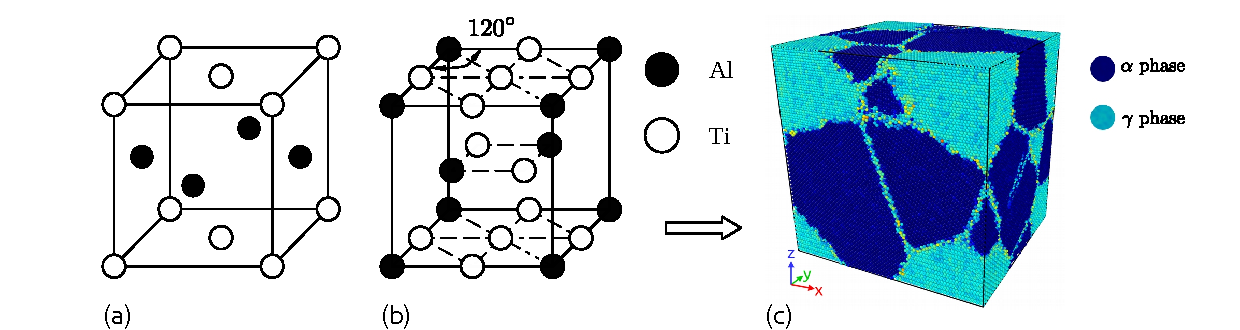
\includegraphics[width=1\linewidth]{img/tial-cell2}
	\caption{Unit cell of \rm{TiAl} (a) and $\rm{Ti_3Al}$ (b)}
	\label{fig:tial-cell}
\end{figure}

\begin{table}[ht]
	\caption{Parameters of nanocrystalline}
	\centering
	\begin{tabular}{c c c l}
	\toprule
	\textbf{Phase}			& {Space group}		& {Designation} 		& {Parameters} \\
	\midrule
	$\alpha_2$ - $\rm{Ti_3Al}$		& $\rm P6_3/mmc$ 	& $\rm 0_{19}$ 		& $a$ = 0.5765 \\
		&					&					& $c$ = 0.46833 \\
	$\gamma$ - $\rm{TiAl}$ 		& $\rm tP4$ 		& $\rm L1_0$		& $a$ = 0.3997 \\
		&					&					& $c$ = 0.4062 \\			
	\bottomrule
	\end{tabular} 
	\label{tab:lattice_parameter}
\end{table} 

$\gamma $ TiAl has a fcc type cell with an $L1_0$ structure, and $\alpha_2 -\rm Ti_3Al$ has a hcp structure, these two types of initial cells are shown in Fig. \ref{fig:tial-cell}, and the constructing parameters are given by Table \ref{tab:lattice_parameter}. Periodic boundary conditions (PBC) are applied along all three directions, that makes poly crystal with periodic nanovoid structures. The initial dimension of simulation cell is $L_x =200$ \si{\angstrom}, $L_y = $180\si{\angstrom}, $L_z = 210$ \si{\angstrom}, and each model contains about 4.6 million atoms. The grain orientation and size were randomly created with Voronoi method by code ATOMSK \cite{Hirel2015}, and resulting in the arbitrary shape and orientation of the grains. Uniaxial load was applied to the model at a strain rate of $5\times10^8\ \rm{s}^{-1}$. 
% In order to study the deformation mechanism of the two phase alloy and the effect of void defect, three types of models were created: Type-1.model without any void defect; Type-2. models with different size void inside $\alpha_2$ phase; Type-3. models with void at $\alpha_2-\gamma$ interface. \ref{tab:lattice_parameter}. The simulation cells of two phase polycrystalline with an initially spherical void at different position are shown in figure .
\subsection{Analysis method}
In order to identify typical defects in the deformed model, a hybrid analysis method was used with free code ovito\cite{Stukowski2010a}.Dislocation is visualized by DXA method, and Centro-symmetry parameter(CSP) is used to tell grain boundary from  $\alpha_2$ phase and $\gamma$ phase. The definition of CSP is as following:

	\begin{equation} \label{eq:csp} 
	P = \displaystyle\sum_{i=1}^{6}|\vec{R_i}+{\vec{R}}_{i+6}|^2
	\end{equation}
	
where $\vec{R_i}$ and ${\vec{R}}_{i+6}$ are the vectors corresponding to the six pairs of opposite nearest neighbors in the fcc lattice. The centro-symmetry parameter(CSP) is zero for atoms in a perfect lattice. In other words, if the lattice is distorted the value of P will not be zero. Instead, the parameter will have a value within the range corresponding to a particular defect. By removing all the perfect and surface atoms within the bulk, the existence of dislocation atoms become visible. 
 
\section{Results and Discussion}\label{section:RD}

\begin{figure}[ht]
	\centering
	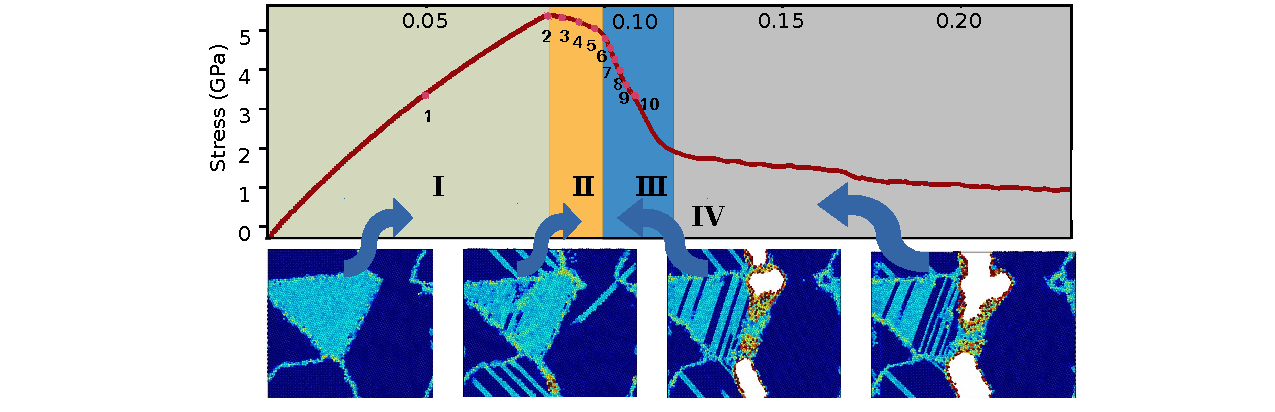
\includegraphics[width=1\linewidth]{img/perfect-line2-2}
	\caption{Deformation process of the model without void defect}
	\label{fig:deformation-pf}
\end{figure}


%	/home/alex/Documents/violet/draft/img/perfect-line.pdf
Deformation process of the model without void defect is shown in Fig. \ref{fig:deformation-pf}. The strength of the model without void defect is 5.3 GPa. According to stress response under constant rate of strain rate, the whole tensile process can be divided into four stages: 
Stage - \uppercase\expandafter{\romannumeral1}: elastic stage,ranging from $\epsilon = 0$ to $\epsilon = 0.092$, including key point 1;
Stage - \uppercase\expandafter{\romannumeral2}: yield stage, ranging from $\epsilon = 0.092$ to $\epsilon = 0.101$, including key points 2 to 6;
Stage - \uppercase\expandafter{\romannumeral3}: cracking stage, ranging from $\epsilon = 0.101$ to $\epsilon = 0.112$, including key pint 7 to 10;
Stage - \uppercase\expandafter{\romannumeral4}: fracture stage. Following discussion concentrates on deformation phenomena that rely on the elastro-plastic codeformation of the $\gamma$ and $\alpha_2$ phases and on the particular point defect situation occurring in two phase alloys. 

\begin{table}[ht]
	\caption{Key points during tensile process}
	\centering
	\begin{tabular}{l c c c c c c c c c c}
		\toprule
		\textbf{Key Number} & {1} & {2} & {3} & {4} & {5} & {6} & {7} & {8} & {9} & {10}\\		 \midrule
		\textbf{Stage} &\uppercase\expandafter{\romannumeral1} &\uppercase\expandafter{\romannumeral1} &\uppercase\expandafter{\romannumeral2} &\uppercase\expandafter{\romannumeral2} &\uppercase\expandafter{\romannumeral2} &\uppercase\expandafter{\romannumeral2} &\uppercase\expandafter{\romannumeral3} &\uppercase\expandafter{\romannumeral3} &\uppercase\expandafter{\romannumeral3} &\uppercase\expandafter{\romannumeral3}\\
		
		\midrule
		% Time/ps	& 0 & 0.15 & 0.16 & 0.17 & 0.18 & 0.19 & 0.Fu = sin20 & 0.21 & 0.22 & 0.23 \\
		% \midule
		\textbf{Strain}	& 0.05 &  0.092 & 0.092 & 0.096 & 0.099 & 0.101 & 0.104 & 0.107 & 0.110 & 0.112 \\
		\bottomrule
	\end{tabular} 
	\label{tab:key-point}
\end{table}

 


% Due to this effect ( $\alpha_2$ + $\gamma$ ) alloys exhibit some remarkable properties that are unlike those of either constituent.
\subsection{Deformation Mechanism of Two Phase TiAl Alloy without Void Defects}
Snapshots of atom configuration at the 5 of 10 key points are shown by Fig. \ref{fig:Defect}.  Atoms with ordered configuration  of $\gamma$ phase grains have been removed in Fig.\ref{fig:Defect}a,\ $\alpha_2$ phase and defects inside grains have been left. Similarly, $\gamma$ phase grain have been removed in Fig. \ref{fig:Defect}b, the defects of $\alpha_2$ phase have been left.  The results show that, at stage \uppercase\expandafter{\romannumeral1}, the structure of the model is under typical elastic deformation and the size of simulation box enlarged due to the loading, deformation of the two phase are compatible. Emission of dislocation and evolution of defects initiated at the end of stage \uppercase\expandafter{\romannumeral1}. A  great number of dislocation emitted inside $\gamma$ phase at stage 2, however, the dislocation inside $\gamma$ phase was emitted after key point 5 shown by Fig. \ref{fig:Defect}b. The deformation of $\alpha_2$ phase is earlier than $\gamma$ phase during yield stage, thus local displacement of two phase are incompatible during yield stage.  



\begin{figure}[ht] 
	\centering
	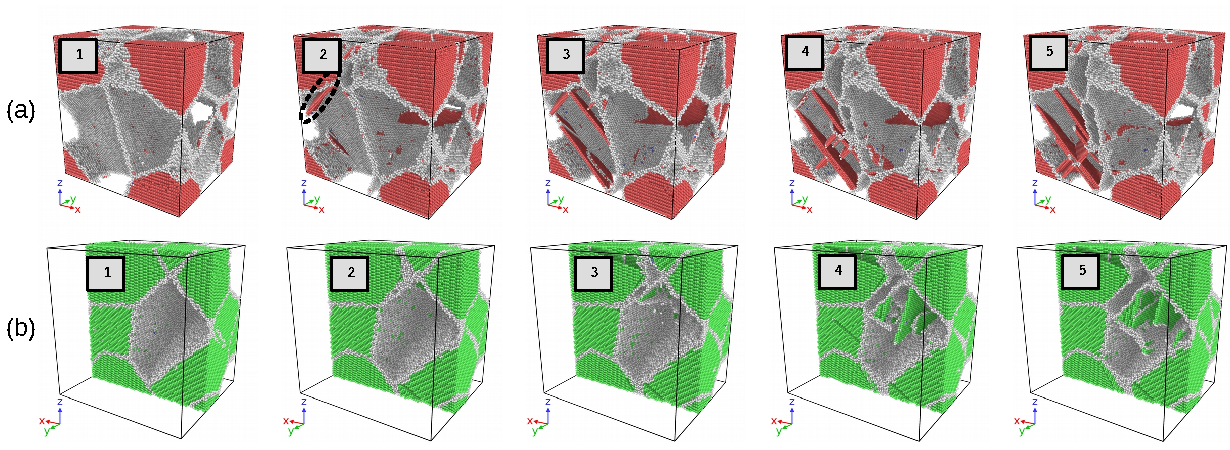
\includegraphics[width=1\linewidth]{img/def2}
	\caption{Microstructure evolution inside $\gamma$ phase(a), $\alpha_2$ phase(b) during yield stage}
	\label{fig:Defect}
\end{figure}

The mobility of dislocation is affected by structure of crystal, loading condition and temperature, and experiments have shown that the velocity of dislocation motion is sensitive to stress and temperature\cite{Stein1960}. The brittleness of two phase Ti-Al alloy attributed to the poor mobility of dislocation at room temperature. Velocity of a screw dislocation can be estimated by Escaig's elastic model \cite{Escaig1968}, it can be written as:
\begin{equation}\label{eq:temp-dis}
v = v_0 \exp(-\Delta H(\tau^*)/kT)
\end{equation}
where the prefactor $v_0$ gives the velocity that would be obtained for each potential mobility, $L$ is the free length of screw character of dislocation, $\Delta H(\tau^*)$ is activation enthalpy determined by loading conditions. The effect of temperature on the mobility can be evaluated under different loading conditions, thus we chose  $\tau_1^*>\tau_2^*>\tau_3^*$ in formulation \ref{eq:temp-dis}, normalized velocity is shown in Fig \ref{fig:temp}. The  velocity  of dislocation movement rise along with increase of  stress, the speed of dislocation is relatively low at 298 K, and it is more sensitive to temperature than shear stress. 


\begin{figure}[ht]
	\centering
	\begin{minipage}{0.495\textwidth}
		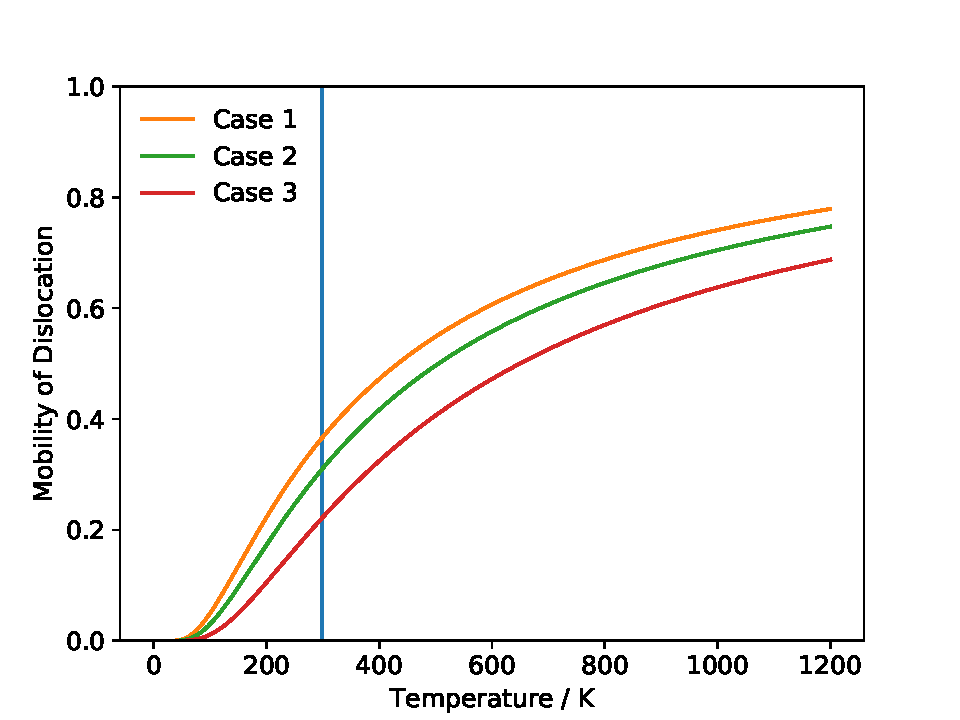
\includegraphics[width=1\linewidth]{img/temp}
		\centering
		\caption{Mobility of dislocation under stress}
		\label{fig:temp}
	\end{minipage}	
	\hfill
	\begin{minipage}{0.495\textwidth}		
		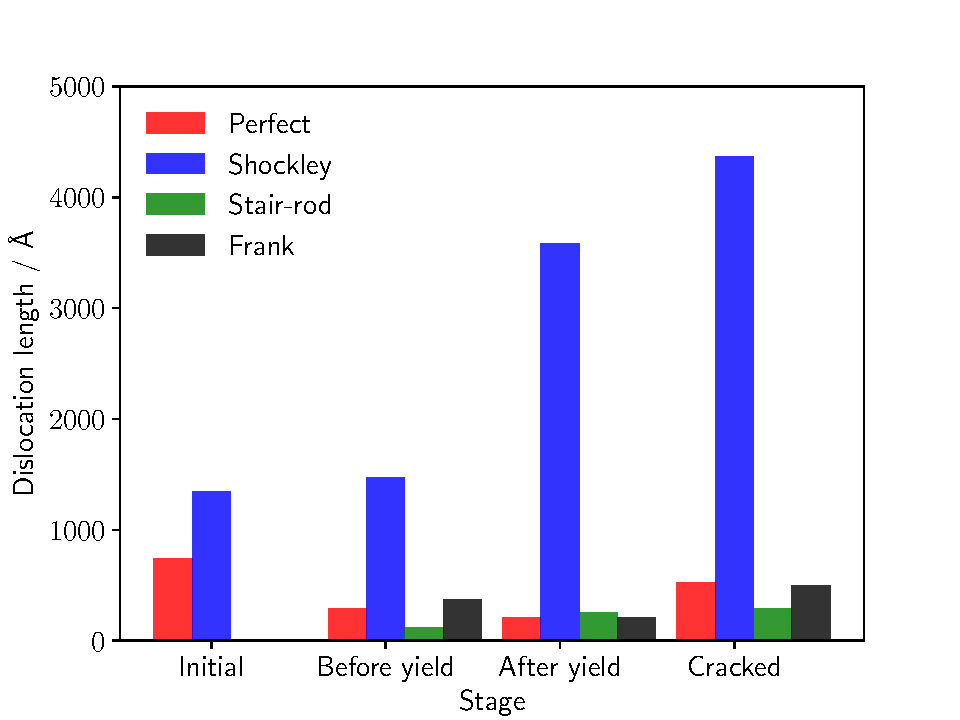
\includegraphics[width=1\linewidth]{img/disum}
		\centering
		\caption{Dislocation length at different stage }
		\label{fig:disum}
	\end{minipage}
\end{figure}


In Fig. \ref{fig:disum}, length of different type dislocation are given at four stages. Dislocations are recognized and identified using the dislocation analysis (DXA) of OVITO. The length of Shorckley dislocation with Burgers vector $1/6[1 1 2]$ increase sharply during yield stage of the deformation process in Fig. \ref{fig:disum}, but the length of perfect dislocation fluctuate at a low level. Decomposition of the perfect  dislocations split into Shockley partial dislocations as formulation \ref{eq:dis-1} and \ref{eq:dis-2}. The structure spontaneously transform into intrinsic stacking fault (ISF), it can be observed in Fig. \ref{fig:Defect}a. 

%\begin{equation}\label{eq:dis-1}
%[\ 0\ 1\ \overline{1}\ ] \to 1/2 [\ 1\ 1\ \overline{2}\ ]+1/2[\ \overline{1}\ 1\ 0\ ]\\
%\end{equation}

\begin{equation}\label{eq:dis-1}
1/2 [\ 0\ 1\ 1\ ] \to 1/6[\ 1\ 1\ 2\ ]+1/6[\ \overline{1}\ 2\ 1\ ]
\end{equation}
\begin{equation}\label{eq:dis-2}
1/2 [\ 1\ 0\ \overline{1}\ ] \to 1/6 [\ 1\ 1\ \overline{2}\ ] + 1/6[\ 2\ \overline{1}\ \overline{1}\ ]
\end{equation}
Interaction between dislocation with Burgers vector of $1/6 [112] $ and $ 1/6 [11\overline{2}]$ follows the decomposition of perfect dislocation. The process produce leading dislocation and a trailing dislocation, when the two leading Shockley partials combine, they form Lomer–Cottrell junction, a separate dislocation. It's sessile and immobile in the slip plane,plays a role of barrier against other dislocations in the plane. The process is as follow :
\begin{equation}\label{eq:dis-3}
1/6 [\ 1\ 1\ 2\ ] + 1/6 [\ 1\ 1\  \overline{2}\ ] \to 1/3 [\ 1\ 1\ 0\ ]
\end{equation}


The orientation of slip is changed in Fig. \ref{fig:Defect}, because the crystallographically available slip and directions are not continuous across the interface. This may significantly reduce the Schmid factor and thus impede slip transfer. At the $\gamma/\gamma$ interfaces, the orientation of slip plan could change through a relevantly large angle of about 90 degree. Reorientation of slip is always required at the $\alpha_{2}/\gamma$ interface; the smallest angle between the corresponding slip planes ${1 1 1}_{\gamma}$ and ${ 1 0 -1 0}_{\alpha_2}$ is about 19 degree \cite{intro-structure}. From Fig. \ref{fig:Defect}, of the two constituents of ($\alpha_2$+$\gamma$) alloys, the $\alpha_2$ phase is more difficult to deform. 

A reason for the unequal strain partitioning between the $\alpha_2$ and $\gamma$ phase is certainly the strong plastic anisotropy of the $\alpha_2$ phase. TEM examinations performed on tensile tested lamellar alloys have revealed that the limited plasticity of the $\alpha_2$ phase is mainly carried by local slip of <a>-type dislocations with the Burgers vector $b=1/3[11\overline{2}0]$ prism planes shown by Fig. \ref{fig:Defect}, which is by far the easiest slip system in $\alpha_2$ single crystals.  The core of a dislocation intersecting an interface often needs to be transformed. For example, an ordinary 1/2[110] dislocation gliding in one $\gamma$ grain has to be converted in to a $[101]$ super dislocation with the double Burgers vector gliding in an adjacent $\gamma$ grain. At the $\alpha_2/\gamma$ interface, dislocations existing in the $D0_{19}$ structure have to be transformed into dislocations consistent with the $L1_0$structure. These core transformations are associated with a change of the dislocation line energy because the lengths of Burgers vectors and the shear module are different. Dislocations crossing semi-coherent boundaries have to intersect the misfit dislocation, a process that involves elastic interaction, jog formation and the incorporation of gliding dislocations into the mismatch structure of the interface.When slip is forced to cross $\alpha_2$ phase, pyramidal slip of the $\alpha_2$ phase is required, which needs an extremely high shear stress.


\subsection{The effect of void on the strength of material}

\begin{figure}[ht]
	\centering
	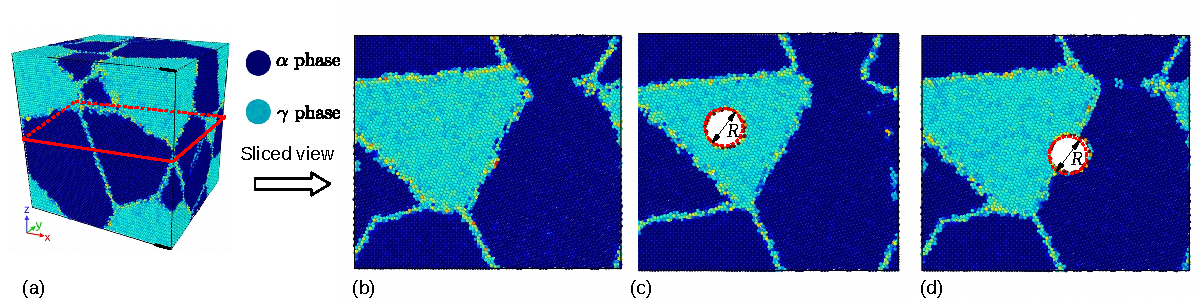
\includegraphics[width=1\linewidth]{img/models}
	\caption{ Model with no void defect (b), with void inside $\alpha_2$ phase (c) with void at $\alpha_2-\gamma$ interface (d)}
	\label{fig:model-creation}
\end{figure}

In Fig. \ref{fig:model-creation}, voids with different size: 2\AA, 5\AA, 10\AA, 15\AA were placed  at $\alpha_2-\gamma$ phase boundary, inside $\gamma$ phase respectively. The strength of materials with void in different size and at different position is shown in Fig.\ref{fig:stress&strain}. The existence of void have little impact on the elastic properties of the material, and the model without void defect has the best strength 5.3 GPa, the yield stress of model with void is smaller. Void at $\alpha_2$-$\gamma$ phase boundary  detracts the strength of  material most, and the void inside $\alpha_2$ phase  have less impact on the strength.          
Conventional definition of strength of materials with geometry subtraction was applied to the model, and theoretical strength of the models was calculated by
\begin{equation} \label{eq:section} 
\sigma^* = \sigma_0 \cdot \frac{A^*}{A_0}
\end{equation}
where $\sigma_0$ is the strength of model without void defects 5.26 Gpa, and $A_0$ is initial section area,  $A^*$ is effective section area.  In classic theory, the relationship between void size and strength of the model is linear. However, simulation results reveals that two phase Ti-Al alloy is sensitive to existence of void defect.  Comparing with the strength determined by molecular dynamics simulation and the result4s calculated with formulation \ref{eq:section}, it can be assumed that the main factor that affects the strength of materials can be attributed to local behavior of the materials, thus revolution of defects should be examined carefully.

\begin{figure}[ht]
	\centering
	\begin{minipage}{0.495\textwidth}
		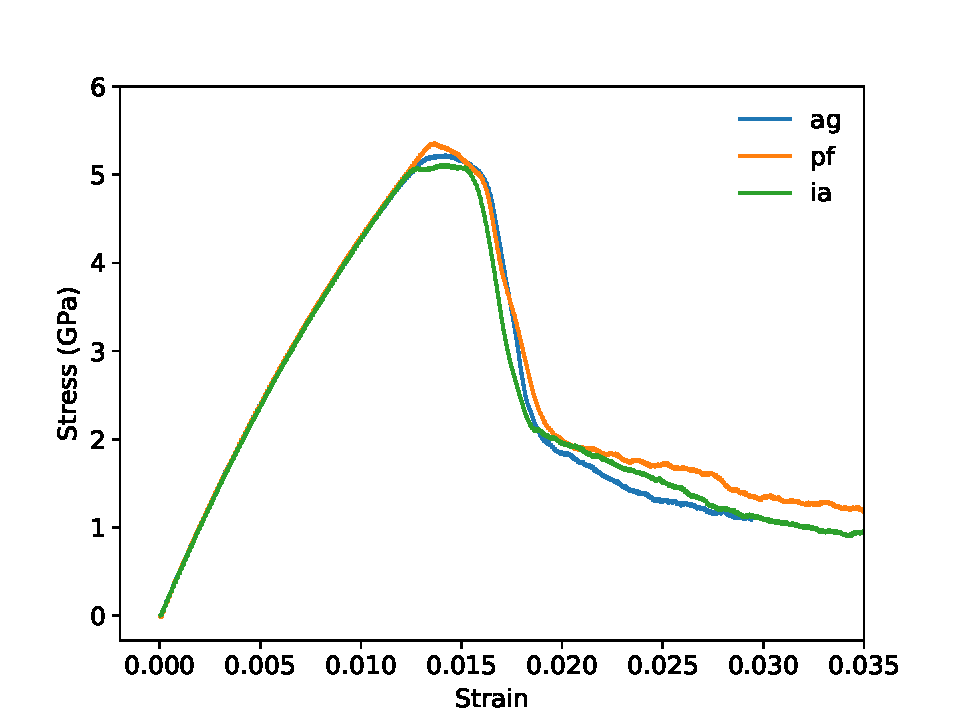
\includegraphics[width=1\linewidth]{img/allline}
		\centering
		\caption{Stress-Strain}
		\label{fig:stress&strain}
	\end{minipage}	
	\hfill
	\begin{minipage}{0.495\textwidth}		
		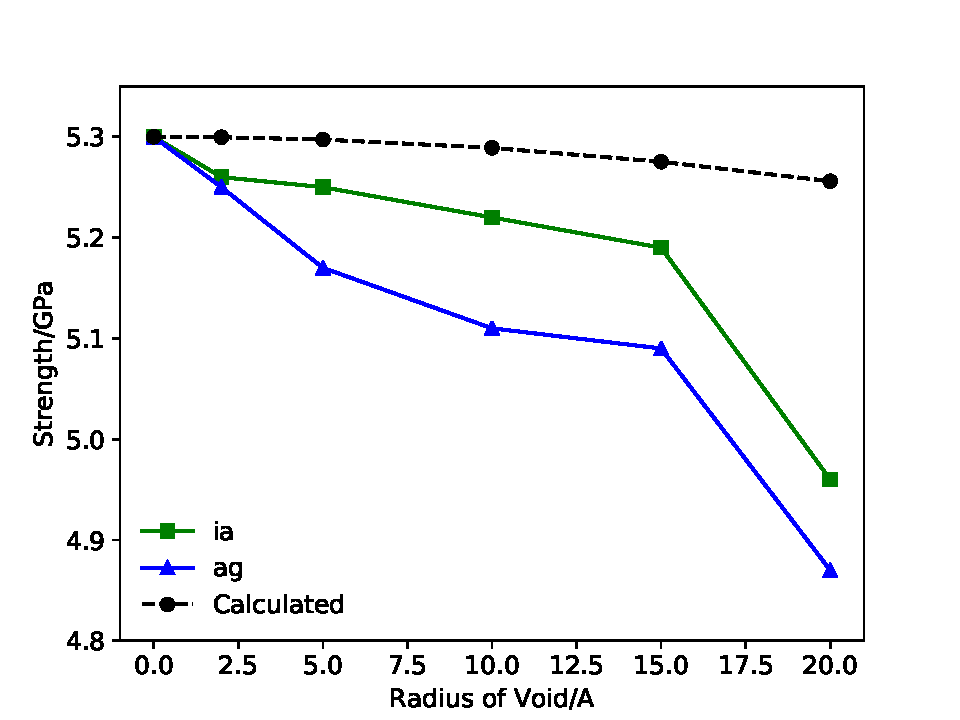
\includegraphics[width=1\linewidth]{img/effect_of_vol}
		\centering
		\caption{Strength of models}
		\label{fig:strength}
	\end{minipage}
\end{figure}


%%%	
%\begin{figure}[ht]
%%	\includegraphics[width=1\linewidth]{"img/fracture3"}
%	\caption{Yield process of the models}
%	\label{fig:yield}
%\end{figure}
	
In Fig. \ref{fig:strength} It has been observed that voids detracts the strengths of  material. The max stress  of the simulation cell decreases as the volume of voids are larger. From Fig \ref{fig:stress&strain}, there is a critical value of void radius about 15 \AA, the void greater than 15 \AA cause serious detraction of strength of material.  The decrease rate of loading area are smaller comparing with the detraction of strength, so it can be assumed that the  yield behavior and strength is much more related with local behavior of grain boundaries and void. Grain and phase boundaries are obstacles to deformation process, thus the stability of boundaries have great impact on the strength of materials. Interactive between grain boundary and void determines the fracture mode of the TiAl alloy.

\subsection{Evolution of spherical void in the simulation with intragranular spherical voids}

\begin{figure}[ht]
	\centering
	\includegraphics[width=1\linewidth]{"img/dis-void2"}
	\caption{Orowan process in $\alpha$-phase ($\alpha$ phase atoms have been removed)}
	\label{fig:orowan}
\end{figure}


The role of void can be concluded as two main parts: source of dislocation and obstacles to dislocations.  Second-phase particles, precipitated within, as a consequence of a thermal treatment, or taken up, as a consequence of a material processing route, into a matrix of the first, dominant phase, disrupt, associated with the occurrence of incoherent or coherent interfaces;the long-range translation symmetry of the matrix. They may induce considerable misfit-stress fields and thus can influence material properties pronouncedly. Such stress fields surrounding the second-phase particles can be due to misfit between the volume occupied by the second-phase particle when unconstrained and the space (“hole”) put at its disposal by the matrix. Such misfit can arise due to specific volume differences induced by precipitation or by different thermal expansion or shrinkage upon heating or cooling the specimen. A possibly favorable effect of second-phase particles is a contribution to the enhancement of mechanical strength. Considering yielding of a material as related to glide of dislocations, any mechanism obstructing dislocation glide improves the mechanical strength. In the discussion of the Frank–Read source for dislocation production  it was made clear that second-phase particles can serve as obstacles for dislocation migration: the stress fields surrounding the second-phase particles can be of block propagation of the stress field of a migrating dislocation: the second-phase particle acts as pinning point. It was already indicated that in order that a dislocation can pass two pinning points a critical shear stress is needed that depends on the distance between  obstacles, which can be regarded as second-phase particles:
\begin{equation} \label{eq:orowan} 
\tau_0 = Gb/d
\end{equation}
where $d$ represents the distance between obstancle A and B , reflects the dependence of the critical shear stress $\tau_0$ on the second-phase particle density and distribution. This mechanism for hardening is designated as the Orowan process with $\tau_0$ as the Orowan (shear) stress.

As a result of the Orowan process, upon passage of the pinning points by a series of gliding dislocations, a system of concentric loops is formed around the second-phase particles. Consequently, the effective average distance between the second-phase particles has decreased to d which implies a necessary increase of the value of critical shear stress required for continuation of dislocation glide. The width of a burgers vector, will be generated at both sides of a crystal along the direction of the burgers vector after dislocation traversing the entire crystal, as is shown in \ref{fig:orowan}. A small tep will be formed at spherical void surface toward the void interior after dislocation absorption at spherical void surfaces. If a great number of dislocation slip along their respective systems towards the spherical nanovoid in all directions, and are absorbed at spherical void surfaces, the spherical nanovoid will eventually shrink from the dash circle 
\section{conclusion}
In this paper, deformation behavior of two phase TiAl alloy under tensile loading was simulated with MD method. The mechanism of deformation was investigated under atomic scale, and the effect of void defect on the properties of two phase TiAl alloy was also studied.  The conclusions are as follows:

(1) The major deformation component of the two phase TiAl alloy is $\gamma$ phase,$\alpha$ phase is harder to be deformed, this inhomogeneity results in cracks at interface of the two phase. 

(2) The effect of the void defect on the strength of the two phase alloy is sensitive to the location of the void. The void located inside the grain decrease the strength to the material because this type defect weaken the grain thus caused even more serious stress concentration, and the void at phase boundary have less impact on the strength of the material because this type void help to release of local stress at grain boundary.


\reftitle{References}
\bibliography{ref/VIOLET-ref.bib}
\funding{This research was funded by the National Natural Science Foundation of China (No. 51665030) and the Program for Changjiang Scholars and Innovative Research Team in Universities of the Ministry of Education of China (No. IRT-15R30) and the Doctoral Research Foundation of Lanzhou University of Technology.}

\end{document}


